
\subsection{Diencephalon}
\label{subsec:Diencephalon} \index{Diencephalon}
%%%%%%%%%%%%%%%%%%%%%%%%%%%%%%%%%%%%%%%%%%%%%%%%%%%%%%%%%%%
%%%%%%%%%%%%%%%%%%%%%%%%%%%%%%%%%%%%%%%%%%%%%%%%%%%%%%%%%%%

Das Diencephalon oder Zwischenhirn befindet sich caudal, bzw. unterhalb des Telencephalons und umschließt den dritten Ventrikel. Es kann in vier Hauptbereiche gegliedert werden. Von superior nach inferior, bzw. dorsal nach rostral, kann zischen \textbf{Epithalamus}, \textbf{Thalamus}, \textbf{Subthalamus}  und \textbf{Hypothalamus} unterschieden werden \textsuperscript{\cite[Kap.~16]{crossman2014neuroanatomy}}.

\subsubsection{Epithalamus}
\label{subsubsec:Epithalamus} \index{Epithalamus}
%%%%%%%%%%%%%%%%%%%%%%%%%%%%%%%%%%%%%%%%%%%%%%%%%%%%%%%%%%%

Der Epithalamus ist ein kleines Teilgebiet des Diencephalons. Er ist dorsal und caudal gelegen. Bekannte Komponenten des Epithalamus stellen die Epiphyse (Abb.~\ref{fig:schaf_midsagittal}~B,D) und die Nuclei habenulares\index{Nuclei! habenulares} (Abb.~\ref{fig:Diencephalon_Ratte}~B-D) dar, die mit dem limbischen System (Kap.~\ref{subsec:limisches_system}) in Verbindung stehen \textsuperscript{\cite[Kap.~12]{crossman2014neuroanatomy}}.\\

\noindent Die \textbf{Epiphyse}\index{Epiphyse} (\textit{Epiphysis cerebri}), auch das \textbf{Pinealorgan} (\textit{Glandula pinealis}) oder die \textbf{Zirbeldrüse}, befindet sich mittig im Diencephalon, direkt rostral des Colliculus superior des Mesencephalons. Bei der Epiphyse handelt es sich um ein unpaares endokrines Organ.
Sie besteht aus Gliazellen und Drüsenzellen, den sogenannten Pinealocyten. Letztere stammen von Photorezeptoren ab und synthetisieren das Hormon Melatonin. Die Epiphyse zeigt, unter anderem  bei einigen Fischen, noch netzhautartige Strukturen auf. Bei Säugern ist jedoch keine Photosensibilität mehr vorhanden. Zudem verliert die Epiphyse bei Säugern nach der Geburt ihre neuronale Verbindung zum Gehirn. Durch die Ausschüttung von Melatonin ist sie in die Regulierung des Schlaf-Wach-Rhythmus involviert und somit an der Steuerung des circadianen Rhythmus beteiligt. Auch bei der Regulation des Einsetzens der Pubertät spielt sie eine wichtige Rolle, sowie bei der Koordination saisonaler Fortpflanzung \textsuperscript{\cite[Kap.~13]{penzlin2005tierphys}}.

\subsubsection{Thalamus}
\label{subsubsec:Thalamus} \index{Thalamus}
%%%%%%%%%%%%%%%%%%%%%%%%%%%%%%%%%%%%%%%%%%%%%%%%%%%%%%%%%%%

Der Thalamus stellt die größte Untereinheit des Diencephalons dar. Gemeinsam mit dem Hypothalamus bildet er die laterale Wand des dritten Ventrikels (Abb.~\ref{fig:Diencephalon_Ratte})  \textsuperscript{\cite[Kap.~12]{crossman2014neuroanatomy}}. \\

\noindent Der Thalamus kann in mehrere kleine Kerngebiete unterteilt werden. Dabei gibt es Nuclei, die sensorische Informationen in die zugehörigen Areale der primären sensorischen Cortices leiten (Abb.~\ref{fig:thalamus_nuclei}) \textsuperscript{\cite[Kap.~12]{crossman2014neuroanatomy}}. Zu diesen Kerngebieten gehören der \textbf{Corpus geniculatum mediale}\index{Corpus! geniculatum mediale} (MGN) und der \textbf{Corpus geniculatum laterale}\index{Corpus! geniculatum laterale} (LGN). Als Station der Hörbahn leitet der MGN auditorische Information vom Colliculus inferior zur Großhirnrinde weiter. Der LGN stellt eine Station der Sehbahn dar, die zwischen der Retina und dem primären visuellen Cortex liegt \textsuperscript{\cite[Kap.~14]{penzlin2005tierphys}}. Des Weiteren können Kerngebiete differenziert werden, die Impulse aus Cerebellum und Basalganglia erhalten und an Motorregionen des Frontallappens gekoppelt sind. Zu dem gibt es Nuclei, die Verbindungen zu assoziativen und limbischen Arealen der Großhirnrinde aufzeigen \textsuperscript{\cite[Kap.~12]{crossman2014neuroanatomy}}.\\
\noindent Im Allgemeinen spielt der Thalamus durch seine reziproken Verbindungen mit dem cerebralen Cortex eine wichtige Rolle für sensorische, motorische und kognitive Funktionen. Er stellt eine obligatorische Umschalt- und Durchgangszentrale sowohl motorischer, als auch sensorischer Bahnen dar (Kap.~\ref{sec:sensorische_Bahnen}) \textsuperscript{\cite[Kap.~6]{storch2012lehrbuchzoo}}.

\begin{figure}[H]
    \centering
    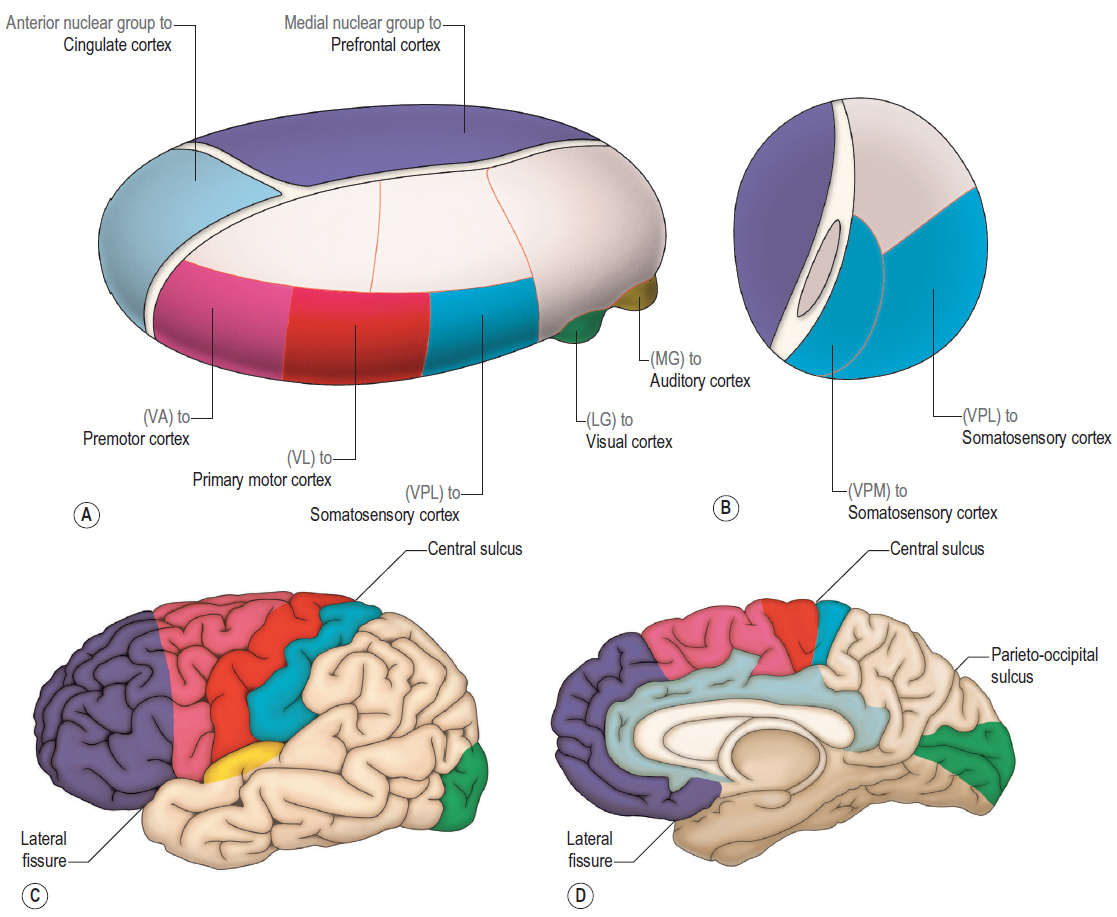
\includegraphics[width=\textwidth]{pictures/Bilder_Jule/Andere/thalamus.png}
    \caption[Projektionen thalamischer Nuclei]{\textbf{Projektionen thalamischer Nuclei.} Dargestellt sind die verschiedenen Teilbereiche des Thalamus des Menschen, sowie die zugehörigen Areale der Großhirnrinde mit denen sie in Verbindung stehen. Zum Thalamus gehören unter anderem der Corpus geniculatum mediale (MGN~- hier MG) und der Corpus geniculatum laterale (LGN~- hier LG). \textbf{A:} anterior-laterale Ansicht, \textbf{B:} Coronalschnitt, \textbf{C:} laterale Ansicht des cerebralen Cortex, \textbf{D:} mediale Aspekte des cerebralen Cortex. Die Farbgebung indiziert die Beziehungen, bzw. Projektionen zwischen den thalamischen Nuclei und den zugehörigen Arealen der Großhirnrinde.\index{Thalamus} Abbildung aus \textit{Neuroanatomy}, Crossman und Neary \textsuperscript{\cite[Kap.~12]{crossman2014neuroanatomy}}.}
    \label{fig:thalamus_nuclei}
\end{figure}

\subsubsection{Subthalamus} \index{Subthalamus}
%%%%%%%%%%%%%%%%%%%%%%%%%%%%%%%%%%%%%%%%%%%%%%%%%%%%%%%%%%%

Der Subthalamus ist eine kleine Region des Diencephalons. In ihm liegt ventro-lateral der subthalamische Nucleus\index{Nucleus! subthalamicus}, direkt medial zur Capsula interna. Er zeichnet sich durch neuronale Verbindungen hin zum Globus pallidus und der Substantia nigra aus. Der subthalamische Nucleus ist an der Kontrolle von Bewegungen beteiligt \textsuperscript{\cite[Kap.~12]{crossman2014neuroanatomy}} und ähnelt somit funktionell den Basalganglia (Kap.~\ref{subsec:basalganglien}) \textsuperscript{\cite[Kap.~16]{crossman2014neuroanatomy}}.

\subsubsection{Hypothalamus}
\label{subsubsec:Hypothalamus} \index{Hypothalamus}
%%%%%%%%%%%%%%%%%%%%%%%%%%%%%%%%%%%%%%%%%%%%%%%%%%%%%%%%%%%

Der Hypothalamus bildet die inferiore, bzw. ventrale Wand des dritten Ventrikels, der vom Diencephalon umgeben wird (Abb.~\ref{fig:Diencephalon_Ratte}). Mittig des Hypothalamus geht das \textit{Infundibulum} hervor, das Hypothalamus und Hypophyse miteinander verbindet. Wie auch der Thalamus besteht der Hypothalamus aus mehreren kleineren Kerngebieten. Dazu gehört der \textbf{Mammillarkörper}\index{Mammillarkörper}, auch \textit{Corpus mamillare} (Abb.~\ref{fig:Diencephalon_Ratte}~A, Abb.~\ref{fig:schaf_MB}), der caudal im Hypothalamus gelegen ist und zum limbischen System (Kap.~\ref{subsec:limisches_system}) gehört \textsuperscript{\cite[Kap.~16]{crossman2014neuroanatomy}}. Beim Menschen, sowie bei Primaten, handelt es sich dabei um eine paarige \textsuperscript{\cite[Kap.~7]{crossman2014neuroanatomy}}, bei anderen Säugetieren, wie der Ratte, um eine unpaare Struktur \textsuperscript{\cite[Kap.~13]{paxinos2014rat}}. Der Mammillarkörper erhält Input aus dem Hippocampus über den Fornix (Abb.~\ref{fig:schaf_midsagittal}~B) und ist an der Regulierung des Gedächtnisses beteiligt \textsuperscript{\cite[Kap.~7]{neurowissenschaften_baer}}. Des Weiteren liegen innerhalb des Hypothalamus neurosekretorische Kerngebiete und die \textbf{Neurohypophyse}\index{Hypophyse! Neurohypophyse}, sowie höhere Koordinationszentren des autonomen Systems \textsuperscript{\cite[Kap.~6]{storch2012lehrbuchzoo}}.

\begin{figure}[H]
    \centering
    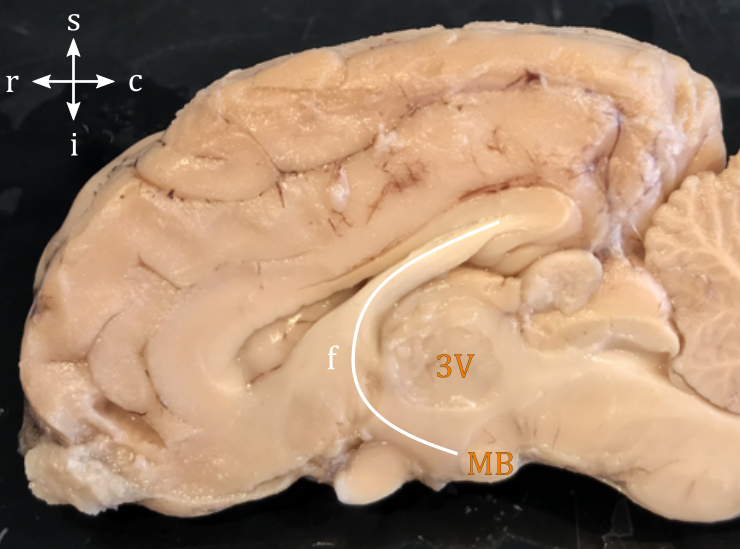
\includegraphics[width=0.5\textwidth]{pictures/Bilder_Jule/Schaf/Ausschnitte/MB.png}
    \caption[Lage der Mammillarkörper]{\textbf{Lage der Mammillarkörper.} Der Mammillarkörper (MB) befindet sich unterhalb des dritten Ventrikels (3V) und steht über den Fornix (f) mit dem Hippocampus in Verbindung.}
    \label{fig:schaf_MB}
\end{figure}{}

\noindent Im Hypothalamus gibt es Thermorezeptoren, die die lokale Temperatur im Hypothalamus wahrnehmen und bei Erwärmung Schwitzen und bei Tieren zudem Hecheln auslösen. Bei Unterkühlung wird Zittern induziert. Osmorezeptoren überwachen die Osmolarität des Blutes, Hormon-Rezeptoren können die Konzentration verschiedener Hormone messen. Dadurch können physiologische Ungleichgewichte erkannt werden, die zu somatosensorischen, vegetativen und endokrinen Reaktionen führen \textsuperscript{\cite[Kap.~14]{penzlin2005tierphys}}. Beispielsweise wirkt sich die Registrierung von Hunger und Durst auf Appetit und Nahrungsaufnahme aus \textsuperscript{\cite[Kap.~6]{storch2012lehrbuchzoo}}. Die vielseitigen Reaktionen, die durch den Hypothalamus gesteuert werden, sind durch seine vielseitigen Projektionen möglich. Sie enden unter anderem im Thalamus, limbischen System, der Hypophyse und dem vegetativen Nervensystem \textsuperscript{\cite[Kap.~16]{crossman2014neuroanatomy}}. \\

\noindent Diese Vielseitigkeit spiegelt sich auch in den Funktionen des Hypothalamus wieder. Zum einen ist er zusammen mit der Hypophyse\index{Hypophyse! allgemein} (Hypothalamus-Hypophysen-System) für wichtige homöostatische Funktionen des Organismus zuständig. Dazu gehört sowohl die Regulation der Körpertemperatur, als auch die des Wasser- und Ionenhaushaltes. Auch ist der Hypothalamus als höchstes Zentrum des vegetativen Nervensystems ein wichtiges Kontrollzentrum für viele Vitalfunktionen \textsuperscript{\cite[Kap.~14]{penzlin2005tierphys}}. Im Allgemeinen ist er in Funktionen des autonomen Nervensystems, des limbischen Systems und des neuroendokrinen Systems involviert \textsuperscript{\cite[Kap.~16]{crossman2014neuroanatomy}}.
 
\begin{figure}[H]
	    \centering
	    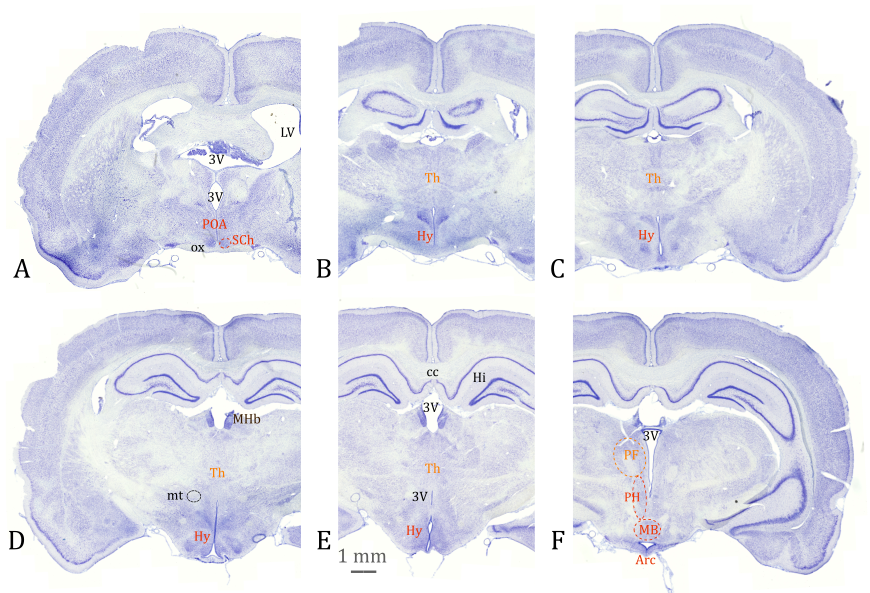
\includegraphics[width=0.99\textwidth]{pictures/Bilder_Jule/Ratte/hypothalamus.png}
	    \caption[Diencephalon Ratte]{\textbf{Diencephalon Ratte.} Gezeigt sind Coronalschnitte des Rattengehirns von rostral nach caudal (A-F: N16-1, N24-4, N24-1, N22-1, N22-1, N20-3). Bereiche des Thalamus (Th) sind in orange gekennzeichnet. Dazu gehört unter anderem der parafascikuläre thalamische Nucleus (PF). Bereiche des Hypothalamus (Hy) sind rot gekennzeichnet. Dem Hypothalamus sind der Mammillarkörper (MB), der Nucleus arcuatus (Arc), sowie der Nucleus suprachiasmaticus (SCh) und das präoptische Areal\index{präoptisches Areal} (POA) untergeordnet. Ebenfalls Teil des Diencephalons sind das optische Chiasma (ox), der dritte Ventrikel (3V), der mammillo-thalamische Trakt (mt), sowie der (mediale) Nucleus habenulares (MHb), der zum Epithalamus gehört. Ebenfalls gekennzeichnet sind Teile des Telencephalons, wie die lateralen Ventrikel (LV), der Hippocampus (Hi) und der Corpus callosum (cc).\index{Thalamus}\index{Hypothalamus}}
	    \label{fig:Diencephalon_Ratte}
\end{figure}{}
